\documentclass[12pt]{article}
\usepackage{mathrsfs}
\usepackage{amsmath,amssymb}
\usepackage{graphicx}
\usepackage[utf8]{inputenc}
\usepackage{amsthm}
\usepackage{tkz-berge}
\usepackage{pgf}
\usepackage{xcolor}
\usepackage{algorithm}
\usepackage{caption}
\usepackage{multicol}
\usepackage{array}
\usepackage[noend]{algpseudocode}
\newcommand{\Term}{Winter 2019}
\newcommand{\Course}{104.272 Discrete Mathematics, Group 1}

\newcommand{\Assignment}{8. Exercise}
\newcommand{\DueDate}{ 4 December, 2019 }

\usepackage[body={6in,9in}]{geometry}



\begin{document}
Hugo \textit{Rincon Galeana}
\begin{center}

\textbf{TU Wien, \Term} \\
\textbf{\Course} (Professor Gittenberger) \\
\textbf{\Assignment, Due \DueDate}
\end{center}


%%%%%%%%%%%%%%%%%%%%%%%%%%%%%%%%%%%%%%%%%%%%%%%%%%%%%%%%%%%%%%%%%%%%%%%%
%% *****      Type your answers after the "\soln" commands      ***** %%
%%%%%%%%%%%%%%%%%%%%%%%%%%%%%%%%%%%%%%%%%%%%%%%%%%%%%%%%%%%%%%%%%%%%%%%%
\begin{enumerate}
    \setcounter{enumi}{70}
    
    \item Prove the following assertions:
        \begin{enumerate}
            \item Every finite lattice has a $0$-element and a $1$-element.
            
            \begin{proof}
            We proceed by induction on the cardinality of the lattice.
            
            \textbf{Base}
            
            The only element in a singleton set $\{x\}$ lattice is both the $0$-element and the $1$-element
            
            \textbf{Induction Hypothesis }
            
            Assume that every finite lattice with $k$ elements has a $0$-element and a $1$-element.
            
            \textbf{Inductive step}
            
            Let $x_1, \ldots, x_{k+1}$ be the elements of the lattice. Notice that $x_1, \ldots, x_k$ form a lattice with $k$ elements. By applying the IH, then there is a $0$-element and an $1$-element for $x_1, \ldots, x_k$. Let $w_0$ be the $0$-element, and $w_1$ the $1$-element. Notice that since $x_1, \ldots, x_{k+1}$ form a lattice, then $w_1 \vee x_{k+1}$ is a 1-element of the whole lattice. Symmetrically $w_0 \wedge x_{k+1}$ is the $0$-element of the whole lattice. 
            
            \end{proof}
            
            \item In every lattice $L$ we have $(x \wedge y) \vee y = y$ for all $x,y \in L$.
            \begin{proof}
                 Notice that from definition $x \wedge y \leq y$, and $(x \wedge y) \vee y \geq y$. Also notice from the definitions of $\wedge $ and $\vee$, that they preserve the partial order on the lattice. Therefore $(x \wedge y) \vee y \leq y \vee y = y$. This implies that $(x \wedge y) \vee y \leq y \leq (x \wedge y)\vee y$. Since the lattice is also a poset, from antisymmetry we have that $y = (x \wedge y)\vee y $
            \end{proof}
            
            \item There exists a lattice such that the following implication is not true:
            $$ x \leq z \Rightarrow  \forall y \; : \; x \vee (y \wedge z) = (x \vee y ) \wedge z$$
            
            \begin{proof}
                Consider the lattice $L$ given by the following Hasse diagram:
                
        \begin{center}
        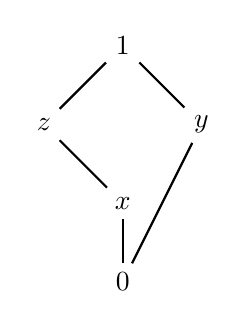
\begin{tikzpicture}
        \node (top) at (0,2) {$1$};
        \node (z) at (-1,1)  {$z$};
        \node (y) at (1,1)  {$y$};
        \node (x) at (0,0)  {$x$};
        \node (bot) at (0,-1) {$0$};
        
        

        
        \draw [black,  thick] (z) -- (top);
        \draw [black,  thick] (y) -- (top);
        \draw [black,  thick] (x) -- (z);
        
        \draw [black,  thick] (bot) -- (x);
        \draw [black,  thick] (bot) -- (y);
        
    \end{tikzpicture}
    \end{center}
            Notice that $y\wedge z = 0$, $x \vee y = 1$, $x \vee (y\wedge z) = x $, $(x \vee y)\wedge z = z$. In this lattice $x \neq z$. Therefore the equation does not hold.
            \end{proof}
            
            
        \end{enumerate}
        

    \item Let $(P, \leq)$ be a finite poset. A subset $C\subseteq P$ is called a \emph{chain} if $(C, \leq)$ is a linearly ordered set. A subset $A \subseteq P $ is called an \emph{antichain} if no two elements of $A $ are comparable with respect to $\leq$. A \emph{chain cover} of $P$ is a partition $P = C_1 \cup C_2 \cup \ldots \cup C_k$ in which all the $C_i$ are chains. Dilworth's Theorem asserts that the size of any largest antichain is equal to the number of chains in a smallest chain cover.
    
    Use Dilworth's Theorem to prove that every poset with at least $rs+1$ elements has either a chain with $r+1$ elements or an antichain with $s+1$ elements.
    
    \begin{proof}
    
    Assume by elimination of the disjunction that there is no antichain with $s+1$ elements in the lattice $L$, therefore if $\mathcal{C}^*$ is an antichain , then it has at most $s$ elements. Notice that the smallest chain cover for $L$ has at most $s$ elements. Let $C_1 , \ldots, C_s$ be the smallest chain cover for $L$. Applying the pigeonhole principle yields that there exists an $i$ such that  $\vert C_i \vert \geq r+1$. Let $C $ be any $r+1$ element subset of $C_i$. Notice that $C$ is a chain of $L$ with $r+1$ elements.
    
    \end{proof}
    
    \item Two numbers $x$ and $y$ are called relatively prime if their greatest common divisor is $1$. Let $p,q,r$ be three distinct prime numbers and $ m = pqr$. How many of the numbers $1,2, \ldots , m$ are relatively prime to $m$.
    
    \begin{proof}
    
    Notice that the numbers that relatively prime to $m = pqr$ are $[m]=\{1,\ldots,m\} \setminus (P \cup Q \cup R)$, where $P$, $Q$ and $R$ are the multiples of $p,q$ and $r$ respectively.
    
    We can compute this by using the inlcusion-exclusion principle for 3 sets (Exercise 70). 
    
    Therefore  $\vert [m]\setminus (P \cup Q \cup R) \vert = m - \vert P \vert - \vert Q \vert - \vert R \vert + \vert P \cap Q \vert + \vert P \cap R \vert + \vert Q \cap R \vert - \vert P \cap Q \cap R \vert $.
    
    Notice that there are $m/p = q \cdot r$ multiples of $p$. Therefore $\vert P \vert = q \cdot r$. Likewise  $\vert Q \vert = p \cdot r$, $\vert R \vert = p \cdot q$.
    
    Also notice that $P \cap Q$ are the numbers that are multiples of both $P$ and $Q$. Since $p$ and $q$ are primes (and therefore relatively primes to each other), then the common multiples of $p$ and $q$ correspond to the multiples of $pq$. This implies that $\vert P \cap Q \vert = \frac{m}{p \cdot q} = r$. By analogy $\vert P \cap R \vert = q$ and $\vert Q \cap R \vert = p$.
    
    Notice that since $p,q,r$ are all primes (and therefore pairwise relatively prime), then the common multiples of $p,q,r$ consist of the multiples of $pqr=m$. There is only $m$ in $P \cap Q \cap R$.
    
    By substituting the inclusion exclusion formula we get that $$\vert [m]\setminus (P \cup Q \cup R) \vert = m- qr -pr - pq +r+ q+ p - 1 $$
    $$ = pqr - qr - pr -pq +r + q + p -1 $$
    $$ = q(r(p-1) + 1)-p(r-q + 1) + r-1 $$
    
    \end{proof}
    
    \item Let $a,b,c,d$ be integers. Prove:
        \begin{enumerate}
            \item If $a | b$ and $a | c$, then for all integers $x,y$ we have a $a | (xb+yc).$
            
            \begin{proof}
                Since $a| b$ , then $a \cdot z_1 = b $. Likewise $a\cdot z_2 = c$ for some $z_1, z_2 \in \mathbb Z$.
                
                Notice that $a(x \cdot z_1 + y \cdot z_2) = x\cdot b + y \cdot c $. This is the definition of $a | (xb+yc)$.
            \end{proof}
            
            \item If $\textrm{gcd}(a,b) = 1 $ and $c|a$ and $d|b$, then $\textrm{gcd}(c,d) = 1$.
                \begin{proof}
                     Let $\textrm{gcd}(c,d) := m$. Then $m|c$ and $m|d$. From the transitivity of $|$ , we have that $m | a$ and $ m | b$. Since $\textrm{gcd}(a,b) = 1$, this implies that $m | 1$. Since the $\textrm{gcd}$ is always a positive number, then $m = \textrm{gcd}(c,d) = 1$ (since the only divisors of 1 are 1 and -1).
                    
                \end{proof}
                
            \item If $a | c$ and $ b | c$ and $\textrm{gcd}(a,b) = 1$, then $ab | c$.
                \begin{proof}
                Notice the equality $\textrm{gcd}(a,b) \cdot \textrm{lcm}(a,b) = p \cdot q$. For this simply consider $a = p_1^{a_1} p_2^{a_2} \ldots p_k^{a_k}$ and $b= p_1^{b_1} p_2 ^{b_2} \ldots p_k^{b_k}$. Notice that $\textrm{gcd}(a,b) = p_1^{min(a_1,b_1)} p_2^{min(a_2,b_2)}\ldots p_k^{min(a_k,b_k)}$. 
                
                Respectively $\textrm{lcm}(a,b) = p_1^{max(a_1,b_1)} p_2^{max(a_2,b_2)}\ldots p_k^{max(a_k,b_k)}$.
                
                Notice that $min(p,q) + max(p,q) = p+q$ for any  $p,q \in \mathbb Z$. Therefore $\textrm{gcd}(a,b) \cdot \textrm{lcm}(a,b) = a \cdot b$ .
                
                Since $\textrm{gcd}(a,b) = 1$, then $\textrm{lcm}(a,b) = a \cdot b$. Notice that $c$ is a common multiple for $a$ and $b$. Therefore $a \cdot b = \textrm{gcd}(a,b) | c$
                \end{proof}
        \end{enumerate}
        
        \item Prove that if $x$ and $y$ are odd integers, then $2 | (x^2 +y^2)$ but $4 \not | (x^2 + y^2)$.
        
            \begin{proof}
                Notice that $x^2$ is odd and $y^2$ is odd, therefore $x^2 + y^2$ is even (divisible by 2).
                
                Notice that $x  \underset{\textrm{mod }4}{\equiv} 1 $ or $x  \underset{4}{\equiv} -1 $ since $x$ is odd. The same applies for $y$.
                
                This implies that $x^2, y^2 \underset{\textrm{mod }4}{\equiv} 1$. Therefore $x^2 + y^2 \underset{\textrm{mod }4}{\equiv} 2$. This shows that $4 \not\vert{x^2+y^2}$
            \end{proof}
            
            \item Prov that for every integer $n$, the number $n^2-n$ is even and $n^3-n$ is a multiple of 6.
            
            \begin{proof}
                Notice that for all $x \in \mathbb Z_2$ $x^2 = x$. This implies that $n^2 \underset{\textrm{mod } 2}{\equiv} n$. Therefore $n^2-n \underset{\textrm{mod }2}{\equiv} 0$. This implies that $n^2-n$ is even.
                
                Notice that in $\mathbb Z_6$ $0 ^3 = 0; 1^3 = 1; 2^3 = 2; 3^3 = 3; 4^3 = 4; 5^3 = 5$. Therefore for all $x \in \mathbb Z_6$, $x^3 = x$. This implies that $n^3 \underset{\textrm{mod }6}{\equiv} n$. This implies that $6 | n^3 -n$.
            \end{proof}
            
            \item Consider two integers $a$ and $b$ such that $\textrm{gcd}(a,4) = 2$ and $\textrm{gcd}(b,4) = 2$. Prove that in this case $\textrm{gcd}(a+b,4)=4$.
            
            \begin{proof}
                Notice that since $\textrm{gcd}(a,4) = 2$, then $4 \not\vert a$. Since $2 \vert a$, then $a \underset{\textrm{mod }4}{\equiv} 2$. The same argument can be repeated for $b$.
                
                Therefore $a+b \underset{\textrm{mod }4}{\equiv} 0$. Therefore $\textrm{gcd}(a+b,4)=4$.
            \end{proof}
            
            \item Prove that any two positive integers $a,b$ satisfy $\textrm{gcd}(a,b) \cdot $
            \begin{proof}
            Consider $a = p_1^{a_1} p_2^{a_2} \ldots p_k^{a_k}$ and $b= p_1^{b_1} p_2 ^{b_2} \ldots p_k^{b_k}$. Notice that $\textrm{gcd}(a,b) = p_1^{min(a_1,b_1)} p_2^{min(a_2,b_2)}\ldots p_k^{min(a_k,b_k)}$. 
                
                Respectively $\textrm{lcm}(a,b) = p_1^{max(a_1,b_1)} p_2^{max(a_2,b_2)}\ldots p_k^{max(a_k,b_k)}$.
                
                Notice that $min(p,q) + max(p,q) = p+q$ for any  $p,q \in \mathbb Z$. Therefore $\textrm{gcd}(a,b) \cdot \textrm{lcm}(a,b) = a \cdot b$ .
            \end{proof}
            
            \item Use the Euclidean algorithm to find two integers $a$ and $b$ such that $420a + 546 b = 42$
            \begin{proof}
            $$546  = 420 \cdot 1 + 126 $$
            $$420 = 126 \cdot 3 + 42$$
            Therefore 
            $42 = 420 -3 \cdot 126$, and $126 = 546 - 1 \cdot 420$
            $$ 42 = 420 - 3 \cdot ( 546 - 1 \cdot 420)$$
            $$ = 4 \cdot 420 - 3 \cdot 546$$
            
            \end{proof}
            
            \item Prove that there exist infinitely many prime numbers $p$ which are solutions of the equation $ p \equiv 3 \textrm{ mod }4$
            
            \emph{Hint: Assume that there are only finitely many such primes, say $p_1, \ldots, p_n$, and consider the number $4p_1p_2\ldots p_n-1$.}
            
            \begin{proof}
                Let $z := 4p_1p_2\ldots p_n-1$. Notice that $4p_1p_2\ldots p_n \underset{\textrm{mod }4}{\equiv} 0$. Therefore $4p_1p_2\ldots p_n-1 \underset{\textrm{mod }4}{\equiv} 3$. Notice that since $4 p_1 \ldots p_n - (4p_1 \ldots p_n -1) = 1$, then $\textrm{gcd}(z,p_i) = 1$.
                
                Therefore $z$ is a product of powers of primes $q_1 \ldots q_m$ such that $\{p_1, \ldots, p_n\} \cap \{q_1, \ldots q_m\} = \varnothing$. Notice that since $p_1 \ldots p_n$ are the only primes that are equivalent to $3$ modulo $4$, then for $i \in \{1, \ldots,m\}$ $q_i \underset{\textrm{mod }4}{\not \equiv} 3$. Also since $z \underset{\textrm{mod }4}{\equiv} 3$, then $i \in \{1, \ldots,m\}$, $q_i \underset{\textrm{mod }4}{\not \equiv} 2,4$. Therefore for all $i \in \{1, \ldots,m\}$, $q_i \underset{\textrm{mod }4}{ \equiv} 1$. Since $z$ is a multiple of only $q_i$ factors, then $z \underset{\textrm{mod }4}{\equiv} 1$. This contradicts that $z \underset{\textrm{mod }4}{\equiv} 3$.
            \end{proof}

\end{enumerate}
    
\end{document}
        
        
    
    
\end{document}